\documentclass[conference]{IEEEtran}
% \IEEEoverridecommandlockouts
% The preceding line is only needed to identify funding in the first footnote. If that is unneeded, please comment it out.

% -----------------
% Packages
% -----------------

\usepackage{amsmath,amsfonts}
\usepackage{algorithmic}
\usepackage{algorithm}
\usepackage{array}
\usepackage[caption=false,font=normalsize,labelfont=sf,textfont=sf]{subfig}
\usepackage{tabularx}
\usepackage{textcomp}
\usepackage{stfloats}
\usepackage{url}
\usepackage{verbatim}
\usepackage{graphicx}
\usepackage{cite}

% -----------------
% Global Defaults
% -----------------

\graphicspath{{figures/}}
% -----------------
% Custom Commands
% -----------------
\newcommand{\R}{\mathbb{R}}
\newcommand{\vect}[1]{\mathbf{#1}}
% -----------------
% Formatting
% -----------------

% \hyphenation{op-tical net-works semi-conduc-tor IEEE-Xplore}

\newcolumntype{Y}{>{\raggedright\arraybackslash}X}

\def\BibTeX{{\rm B\kern-.05em{\sc i\kern-.025em b}\kern-.08em
    T\kern-.1667em\lower.7ex\hbox{E}\kern-.125emX}}


% updated with editorial comments 8/9/2021

\begin{document}

\title{Dual-System Human-Centric Recommender with Fatigue-Aware Long-Term Optimization (DS-HCRS)

% Small text below title
% {\footnotesize \textsuperscript{*}Note: Sub-titles are not captured in Xplore and should not be used}

% Small text below first column
% \thanks{Identify applicable funding agency here. If none, delete this.}

}

\author{
        \IEEEauthorblockN{1\textsuperscript{st} Anirudh Sharma}
        \IEEEauthorblockA{
                \textit{M.Tech. in Artificial Intelligence and Data Science} \\
                \textit{International Institute of Information Technology}\\
                Bangalore, India \\
                % email address or ORCID
        }
        \and
        \IEEEauthorblockN{2\textsuperscript{nd} Shreya Gupta}
        \IEEEauthorblockA{
                \textit{M.Tech. in Artificial Intelligence and Data Science} \\
                \textit{International Institute of Information Technology}\\
                Bangalore, India \\
                % email address or ORCID
        }
}

\maketitle

\begin{abstract}
Recommender systems are often designed to optimize for metrics such as click-through rates and interaction frequency.
These signals are easy to measure, but they only reflect short-term engagement statistics and may not always reflect long-term user satisfaction.
Optimising heavily on short term engagement leads to repetitive recommendations, cognitive fatigue, and reduced user interest, which further leads to reduced engagement with the platform.
This work explores the design of a Dual-System Human-Centric Recommender System (DS-HCRS) that balances short-term engagement with long-term user experience.
The framework combines a fast sequential recommender for immediate relevance with a component that attempts to model long-term user satisfaction.
This long-term component attempts to model the fatigue and discontentment states in a user based on interaction history, which helps create an estimate of boredom or dissatisfaction states.
Furthermore, this component also attempts to model changes in preference of the user over time.
This allows the system to adapt its recommendation strategy accordingly to establish a balance between short and long term goals of user retension.
% The proposed evaluation framework includes both traditional ranking metrics and additional measures related to diversity, novelty, and user engagement on social media datasets.
\end{abstract}

\begin{IEEEkeywords}
Recommender Systems, Long-Term Optimization, Reinforcement Learning,
User Fatigue, Cognitive State Modeling, Dynamics of Preference,
Sequential Recommendation
\end{IEEEkeywords}

\section{Introduction}

Recommender systems have evolved from early accuracy-focused algorithms 
to complex industrial systems across e-commerce, media, and social platforms.
Despite these advances, a tension exists between short-term business-driven goals and long-term user wellbeing.
Most current systems rely on easily measurable signals like clicks and watch time, 
which maximize immediate engagement but often do not explicitly model the user's cognitive state.

\subsection*{The Challenge of Engagement Bias}

Standard sequential and deep learning models treat user histories as ordered sequences to predict the next likely interaction.
While effective at capturing recency effects, these models implicitly assume that maximizing immediate clicks corresponds to maximizing satisfaction.
This approach neglects psychological factors such as \textbf{fatigue} and \textbf{diminishing utility}, 
where repeated exposure to similar content reduces its value and this leads to platform disengagement.

\subsection*{Proposed Solution: DS-HCRS}

To address these limitations, this work proposes a framework called \textbf{DS-HCRS} 
which goes beyond a single static strategy by incorporating:

\begin{itemize}
    \item \textbf{Dual-System Architecture:} Balancing a fast "impulsive" model for relevance with a reflective "long-term" optimizer.
    \item \textbf{Dynamics of Preference:} Estimating changes in user preference using recurrent models.
    \item \textbf{Cognitive State Modeling:} Estimating user fatigue and discontentment using Reinforcement Learning objectives.
\end{itemize}

These three systems alone allows the algorithm to implement more complex systems like 
updating user preference (embeddings) on the go, and cold start handling for new users and items.
By framing recommendation as a cognitive process rather than just a prediction problem,
we aim to develop systems that are sustainable, adaptive, and better aligned with long-term user experience.

% \section{Foundations and Background Concepts}

\section{Literature Survey}

\textbf{PLANNER}

This should NOT be paper-by-paper summaries.
Instead organize by research themes.

\subsection{Engagement-Optimized Recommender Systems}

Survey:

\begin{itemize}
    \item deep ranking models
    \item click prediction frameworks
\end{itemize}   

Findings:

\begin{itemize}
    \item short-term bias
    \item reward misalignment
\end{itemize}
    
\subsection{Sequential \& Session-Based Recommendation}

Focus:

\begin{itemize}
    \item temporal dynamics    
    \item user behavior modeling
\end{itemize}   

Limitation:

\begin{itemize}
    \item no cognitive saturation modeling.
\end{itemize}

\subsection{Reinforcement Learning for Long-Term Optimization}

Include:

\begin{itemize}
    \item contextual bandits    
    \item long-horizon RL papers
    \item welfare-aware RL
\end{itemize}
    
Findings:

\begin{itemize}
    \item reward definition still engagement-heavy.
\end{itemize}
    
\subsection{Human-Centered and Welfare-Aware Recommenders}

Discuss:

\begin{itemize}
    \item System-2 recommenders
    \item user satisfaction modeling
    \item ethical optimization
\end{itemize}
    
Key insight:  
$\Rightarrow$ theory exists, integration missing.

\subsection{Bias, Manipulation, and Overconsumption Studies}

From SemanticScholar papers:

\begin{itemize}
    \item addictive interaction dynamics
    \item divisive content amplification
    \item welfare tradeoffs    
\end{itemize}    

\subsection{LLM-Augmented Recommender Systems}

Themes:

\begin{itemize}
    \item semantic reasoning    
    \item concept embeddings
    \item controllable recommendation
\end{itemize}    

Gap:

\begin{itemize}
    \item reasoning used for relevance, not wellbeing.
\end{itemize}
    
\subsection{Key Trends from Major Conferences}

(Summarize trends rather than papers)

From:

\begin{itemize}
    \item RecSys 2024/2025
    \item SIGIR 2024
    \item KDD 2024
\end{itemize}
    

Observed shifts:

\begin{itemize}
    \item long-term evaluation
    \item controllability
    \item explainability
    \item hybrid AI systems
\end{itemize}

\subsection{Literature Synthesis Table (VERY IMPORTANT)}

Create table:

\begin{table}[!t]
\caption{An Example of a Table\label{tab:tableABC}}
\centering
\begin{tabular}{|l||c||c||c||c|}
\hline
Category & Representative Work & Objective & Strength & Limitation \\
\hline
Value 1 & Value 2 & Value 3 & Value 4 & Value 5 \\
\hline
\end{tabular}
\end{table}

This becomes your strongest survey artifact.

% \section{Problem Identification}

The literature survey highlights several limitations, a result of how these systems are designed and evaluated.
Current approaches prioritize short-term engagement and observable signals, often ignoring aspects 
like the human behavior (cognition, preferences, and satisfaction).
These limitations also lead to unintended consequences such as user fatigue, repetitive recommendations, 
and declining long-term engagement.

This section summarizes the key problems identified in the literature survey 
and motivates the need for a more human-centered recommendation framework.

%%%%%%%%%%%%%%%%%%%%%%%%%%%%%%%%%%%%%%%%%%%%%%%%%%%%%%%%%%%%%%%%
%%%%%%%%%%%%%%%%%%%%%%%%%%%%%%%%%%%%%%%%%%%%%%%%%%%%%%%%%%%%%%%%

\subsection{Short-Term Engagement Bias}

The focus on immediate user interaction has heavily influenced the design toward 
metrics like click-through rate (CTR), watch time, or the probability that a user
will interact with the next recommended item.
While these metrics are easy to measure and optimize for; they primarily represent 
short-term engagement rather than long-term satisfaction.

A recommendation that successfully triggers a click does not necessarily mean that
the user found it valuable or enjoyable; which in turn does not guarantee their 
retension over an extended period of time.
Additionally, users may interact with content out of curiosity rather than genuine interest.

Because of this, many recommendation algorithms are trained to 
maximize short-term interactions rather than long-term user value.
Over time, this can encourage content that attracts attention 
quickly but may not contribute satisfying user experiences.

This creates a bias in recommendation systems: \textbf{the system becomes optimized for immediate engagement rather than sustainable user satisfaction.}

%%%%%%%%%%%%%%%%%%%%%%%%%%%%%%%%%%%%%%%%%%%%%%%%%%%%%%%%%%%%%%%%
%%%%%%%%%%%%%%%%%%%%%%%%%%%%%%%%%%%%%%%%%%%%%%%%%%%%%%%%%%%%%%%%

\subsection{Lack of Cognitive State Modeling}

Traditional algorithms of recommendation work around 
available historical data about the user interactions.
In these models, a user is typically represented as 
a sequence of past clicks, views, or purchases.

This approach is effective for identifying behavioral patterns; however, it treats users 
as static data sources, completely ignoring their changing mental states and intentions.
Important psychological factors such as attention, curiosity, 
boredom, and fatigue does not have an explicit representation in the model.

As a result, the system can observe \textit{what users do}, but it 
cannot infer \textit{how users feel} about their current experience.
For example, a user who continues interacting with recommendations might appear 
highly engaged, even if they are becoming tired of the repetitive content.

Without modeling a cognitive state, recommender systems lack the ability to adapt 
to a strategy which can work around how users are experiencing the process.

%%%%%%%%%%%%%%%%%%%%%%%%%%%%%%%%%%%%%%%%%%%%%%%%%%%%%%%%%%%%%%%%
%%%%%%%%%%%%%%%%%%%%%%%%%%%%%%%%%%%%%%%%%%%%%%%%%%%%%%%%%%%%%%%%

\subsection{Absence of Fatigue and Diminishing Utility}

Another important limitation observed is the assumption that 
user utility remains constant across repeated interactions.
Most models assume that if a user interacted with some content in the past, 
recommending similar items repeatedly is a good move.

However, in reality, this repeatition often leads to \textit{diminishing utility}.
As users encounter similar recommendations multiple times, 
the perceived value of those recommendations decreases.
This leads to boredom, reduced interest, and eventually disengagement.

For example, if a user is recommended several videos from a single category or receives
similar product recommendations, the novelty of those recommendations gradually declines.
Despite that, many models continue to reinforce the same patterns 
because they rely heavily on past interaction signals.

Since this notion of fatigue is not explicitly modeled, recommender systems 
unintentionally generate overly repetitive recommendation streams.

%%%%%%%%%%%%%%%%%%%%%%%%%%%%%%%%%%%%%%%%%%%%%%%%%%%%%%%%%%%%%%%%
%%%%%%%%%%%%%%%%%%%%%%%%%%%%%%%%%%%%%%%%%%%%%%%%%%%%%%%%%%%%%%%%

\subsection{Static Recommendation Policies}

Most model from the traditional setting learn a single strategy representing the training data.
Therefore, given the historical pretext, these models perform really well.
Unfortunately, a user is a dynamic entity, with evolving flavours and tastes.
A single strategy is insufficient to keep track of a user's state or context.

This means the system is incapable of dynamically adjusting its decision strategy 
based on factors such as session length, user exploration patterns, or signs of fatigue.
Once a ranking model is trained, it is used to generate recommendations in the same way for every interaction.

In practice, different situations may require different recommendation strategies.
Early in a session, users may prefer familiar and relevant content.
Later in the session, introducing novelty or diversity might help prevent fatigue.

Since current systems typically rely on static ranking policies, they lack 
the ability to adapt its strategy to changing user cognitive state.

%%%%%%%%%%%%%%%%%%%%%%%%%%%%%%%%%%%%%%%%%%%%%%%%%%%%%%%%%%%%%%%%
%%%%%%%%%%%%%%%%%%%%%%%%%%%%%%%%%%%%%%%%%%%%%%%%%%%%%%%%%%%%%%%%

\subsection{Misaligned Evaluation Metrics}

Evaluation metrics play a critical role in shaping recommender system design.
Most systems are evaluated using metrics such as Precision@K, Recall@K, and 
NDCG; these metrics measure how accurately the system predicts user interactions.

These metrics are useful for benchmarking algorithm performance, however, 
only for predictive accuracy, rather than long-term user outcomes.
A system with a high ranking accuracy can still produce 
repetitive content, thus reducing user satisfaction.

Furthermore, offline evaluation methods often fail to capture the dynamic 
feedback loops that take place with real user interactions over time.
As a result, models that perform well in offline experiments 
may not always produce the best long-term user experiences.

%%%%%%%%%%%%%%%%%%%%%%%%%%%%%%%%%%%%%%%%%%%%%%%%%%%%%%%%%%%%%%%%
%%%%%%%%%%%%%%%%%%%%%%%%%%%%%%%%%%%%%%%%%%%%%%%%%%%%%%%%%%%%%%%%

\subsection{Summary of Identified Problems}

The analysis above highlights several key limitations in current recommender system design:

\begin{table}[h]
\caption{TODO Add a caption\label{tab:TODOlabel0102526}}
\centering
\begin{tabularx}{\columnwidth}{|l||Y|}
\hline
Problem & Description \\
\hline
Short-term engagement bias & Systems prioritize immediate interactions rather than long-term satisfaction \\
Lack of cognitive state modeling & Users are represented only through behavior sequences \\
Absence of fatigue modeling & Repeated recommendations may reduce user interest over time \\
Static recommendation policies & Systems do not adapt strategies based on user state \\
Misaligned evaluation metrics & Metrics reward interaction prediction rather than user wellbeing \\
\hline
\end{tabularx}
\end{table}

Together, these limitations suggest that current recommender systems are primarily optimized for \textbf{short-term behavioral signals rather than long-term human-centered outcomes}.

These challenges motivate the development of new recommendation frameworks that can explicitly consider user cognitive state, fatigue, and long-term satisfaction when generating recommendations.


\section{Proposed Methodology: DS-HCRS Framework}

\textbf{PLANNER}

(Conceptual - no implementation details.)

\subsection{Design Philosophy}

Principles:

\begin{itemize}
    \item human-aware optimization
    \item adaptive cognition modeling
    \item long-term value
\end{itemize}
    
\subsection{System Overview Architecture}

High-level diagram description:

User → State Modeling → Dual Systems → Gating → Recommendation → Feedback.

\subsection{System 1: Fast Engagement Model}

Role:

\begin{itemize}
    \item reactive ranking
    \item immediate reward modeling.
\end{itemize}
    
\subsection{Fatigue \& Cognitive Burden Model}

Define variables:

\begin{itemize}
    \item repetition
    \item entropy decay
    \item session length
    \item novelty loss
\end{itemize}    

Explain theoretical grounding.

\subsection{System 2: Reflective Long-Term Optimizer}

Conceptual RL formulation.

Explain:

\begin{itemize}
    \item delayed reward
    \item retention proxy
    \item welfare regularization.
\end{itemize}    

\subsection{Dual-System Gating Mechanism}

Decision policy rationale.

Explain adaptive reasoning depth idea.

\subsection{Optional Concept Embedding Module}

LLM embeddings for cold start.

\subsection{Learning Objective Formulation}

General reward:

\[
R_t = \alpha E_t + \beta L_t - \gamma F_t
\]

Explain meaning conceptually.

\subsection{Expected Advantages Over Existing Systems}

Table comparison:

\begin{table}[!t]
\caption{An Example of a Table\label{tab:table1}}
\centering
\begin{tabular}{|l||c||c|}
\hline
Feature & Traditional & Proposed \\
\hline
Fatigue modeling & cross & tick \\
Long-term reward & Partial & Explicit \\
Adaptive reasoning & cross & tick \\
\hline
\end{tabular}
\end{table}
\section{Evaluation Design}

\textbf{PLANNER}

(No experiments yet.)

\subsection{Baseline Models}

\begin{itemize}
    \item sequential recommender
    \item RL recommender
\end{itemize}

\subsection{Metrics}

\subsubsection{Short-term}

\begin{itemize}
    \item NDCG
    \item Recall@K
\end{itemize}

\subsubsection{Long-term}

\begin{itemize}
    \item retention proxy
    \item churn delay
    \item fatigue score
\end{itemize}

\subsection{Simulation Framework}

Explain trajectory simulation conceptually.

\subsection{Ablation Philosophy}

Why component removal validates design.

% \section{Expected Research Contributions}

EVERYTHING IS A I HERE, NEEDS REWRITING

The proposed Dual-System Human-Centric Recommender System (DS-HCRS) introduces several conceptual and methodological contributions to the design of recommender systems.
While the implementation and empirical evaluation are planned for future work, the proposed framework outlines a structured approach for incorporating cognitive modeling and long-term optimization into recommendation pipelines.

The expected contributions of this work can be summarized as follows.

\subsection{Dual-System Recommendation Architecture}

This work proposes a dual-system recommender architecture inspired by cognitive theories of human decision-making.
The framework separates recommendation strategies into two complementary components:

\begin{itemize}
    \item \textbf{System 1}, which captures short-term behavioral preferences and predicts immediate user interactions.
    \item \textbf{System 2}, which evaluates recommendations using longer-term utility signals and broader contextual information.
\end{itemize}

By explicitly separating impulsive interaction prediction from reflective optimization, the proposed system introduces a structured way to balance short-term engagement with long-term user outcomes.
This architectural design provides a flexible framework that can integrate different recommendation models while maintaining a clear conceptual separation of objectives.

\subsection{Fatigue-Aware Recommendation Modeling}

Another key contribution of this work is the introduction of an explicit \textit{user fatigue and cognitive state model} within the recommendation pipeline.

Traditional recommender systems assume that additional user interactions always indicate positive engagement.
However, prolonged sessions and repeated exposure to similar content may lead to boredom or cognitive overload.
The proposed fatigue modeling component attempts to estimate this state using observable interaction signals such as repetition, novelty, and session length.

By incorporating fatigue estimates into the recommendation process, the system can adapt its behavior when signs of declining user interest are detected.

\subsection{Adaptive Strategy Selection Through Gating}

The proposed system introduces an adaptive gating mechanism that dynamically determines how recommendations from different components should be combined.

Instead of relying on a single recommendation strategy for all situations, the system adjusts the influence of System 1 and System 2 based on the user's current interaction context.
This adaptive decision process allows the recommender to maintain efficiency during normal usage while introducing more reflective reasoning when the user's experience begins to deteriorate.

Such adaptive control mechanisms provide a potential pathway toward more context-aware recommender systems.

\subsection{Integration of Long-Term Utility Optimization}

The proposed framework incorporates long-term optimization principles into the recommendation pipeline by modeling recommendations as sequential decisions that influence future user behavior.

By combining short-term engagement signals with longer-term indicators such as retention and fatigue, the framework outlines a multi-objective reward structure that can guide recommendation policies toward more sustainable outcomes.

This integration highlights how reinforcement learning-based ideas can be used to move beyond purely engagement-driven recommendation objectives.

\subsection{Human-Centered Evaluation Perspective}

Finally, this work proposes an evaluation framework that extends beyond traditional recommendation accuracy metrics.
In addition to standard ranking measures, the evaluation strategy includes metrics related to diversity, novelty, fatigue indicators, and long-term engagement.

This broader evaluation perspective aligns the system with recent research directions in human-centered recommender systems and responsible AI.
By incorporating metrics related to user experience and cognitive load, the proposed evaluation framework aims to provide a more comprehensive understanding of recommender system behavior.

Overall, the proposed framework contributes a structured approach for combining behavioral prediction, cognitive modeling, and long-term optimization within a single recommender system architecture.
The design emphasizes adaptability and human-centered objectives while remaining compatible with existing recommendation techniques.


% \section{Limitations and Ethical Considerations}

\textbf{PLANNER}

Very important academically.

Discuss:

\begin{itemize}
    \item proxy wellbeing limitations
    \item offline evaluation constraints
    \item simulation assumptions
    \item ethical deployment risks
\end{itemize}
% \section{Future Research Directions}

\textbf{PLANNER}

Examples:

\begin{itemize}
    \item real user studies
    \item adaptive psychological modeling
    \item causal preference learning
    \item multi-user ecosystem welfare
\end{itemize}
\section{Results and Analysis}

\subsection{Core Recommendation Metrics}

Fig.~\ref{fig:core_metrics} shows the performance of different models across multiple interaction stages (T0, T100, T300, T500).
These stages represent how the system behaves as more user interaction history becomes available.

\begin{figure*}[!h]
\centering
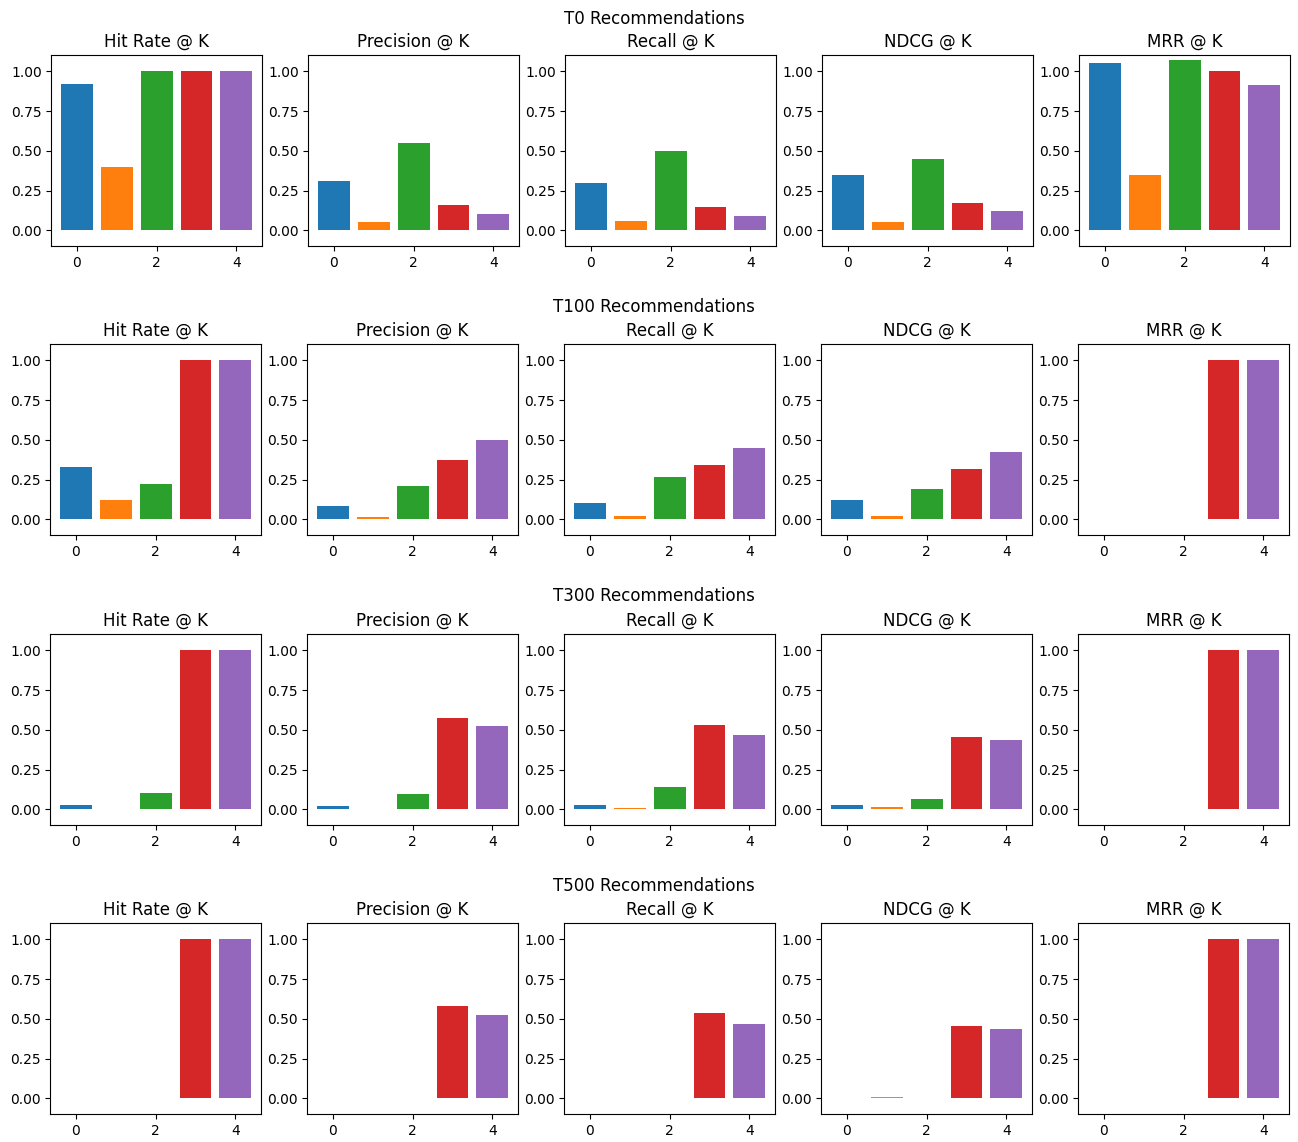
\includegraphics[width=\textwidth]{../figures/core metrics.png}
\caption{Performance comparison of all models across different interaction stages (T0, T100, T300, T500). Static models such as ALS and S1 perform well at early stages but degrade as user preferences evolve. In contrast, S2P and S2F improve over time by adapting to interaction history, with S2F showing a slight trade-off in accuracy due to cognitive-state-aware recommendations.}
\label{fig:core_metrics}
\end{figure*}

\subsubsection{Performance at Initial Stage (T0)}

At T0, where no interaction history is available, the \textbf{S1 model performs the best across all accuracy and ranking metrics}. 
This is expected, since S1 is trained on static user preferences and is specifically designed for this scenario.

On the other hand, both \textbf{S2P and S2F perform relatively poorly at this stage}.
These models rely on interaction history to update user preferences,
and in the absence of such history, they do not have enough information to perform well.

This shows that \textbf{static models are strong in cold-start or early-stage scenarios}.

\subsubsection{Effect of Preference Dynamics (T100 to T300)}

As interaction history increases, a clear shift in performance can be observed.

The performance of \textbf{S1 drops significantly} across all metrics. 
This indicates that static embeddings quickly become outdated when user preferences start evolving.

In contrast, \textbf{S2P shows a strong improvement} in all metrics. 
Since it updates user embeddings using interaction history, it is able to track preference changes effectively. 
As a result, it outperforms all static and classical models in mid and later stages.

This demonstrates the importance of \textbf{modeling preference dynamics instead of relying on fixed embeddings}.

\subsubsection{Effect of Cognitive Modeling (S2P vs S2F)}

When comparing S2P and S2F, an interesting pattern emerges.

S2P achieves \textbf{slightly higher values in precision, recall, and NDCG}, indicating that it is more focused on recommending highly relevant items.

However, S2F performs slightly lower on these metrics. 
This is expected, since S2F does not purely optimize for relevance. 
Instead, it balances:

\begin{itemize}
    \item Relevance
    \item Fatigue
    \item Discontentment
\end{itemize}

Because of this, S2F occasionally introduces less relevant or more diverse items, which slightly reduces short-term accuracy.

This highlights an important trade-off:

\textbf{Optimizing only for relevance (S2P) leads to better short-term accuracy, while incorporating cognitive factors (S2F) leads to more balanced and sustainable recommendation behavior.}

\subsubsection{Long-Term Behavior (T300 to T500)}

At later stages, both S2P and S2F achieve very high performance, with:

\begin{itemize}
    \item Hit Rate approaching 1
    \item MRR close to 1
\end{itemize}

This means that \textbf{relevant items are almost always present, and often appear at the top of the recommendation list}.

Meanwhile, S1 continues to degrade, and classical methods like ALS and BPR fail to adapt to changing preferences.

This further reinforces that:

\textbf{Static and traditional models are not suitable for dynamic recommendation environments.}


%%%%%%%%%%%%%%%%%%%%%%%%%%%%%%%%%%%%%%%%%%%%%%%%%%%%%%%%%%%%%%%%
%%%%%%%%%%%%%%%%%%%%%%%%%%%%%%%%%%%%%%%%%%%%%%%%%%%%%%%%%%%%%%%%

\subsection{Simulation Metrics}

The second set of results focuses on the simulated behavior of the user, rather than only the ranking quality of the recommender. 
These metrics are important because our system is not just trying to recommend relevant items. 
It is also trying to control fatigue, avoid discontentment, and keep the interaction healthy over time. 
Fig.~\ref{fig:simulation_metrics} shows four key behavioral metrics: return rate, acceptance rate, time to boredom, and coverage.

\begin{figure*}[!h]
\centering
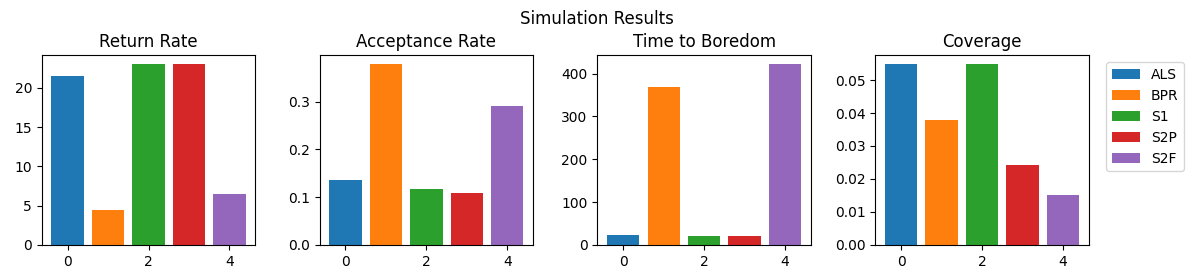
\includegraphics[width=\textwidth]{../figures/simulation metrics.png}
\caption{Comparison of behavioral metrics including return rate, acceptance rate, time to boredom, and coverage. While relevance-driven models (ALS, S1, S2P) lead to quicker fatigue, S2F significantly increases time to boredom by balancing relevance and diversity. The coverage trends highlight the interaction between recommendation behavior and evolving user preference within the simulation.}
\label{fig:simulation_metrics}
\end{figure*}

\subsubsection{Behavioral Trade-offs Across Models}

A clear pattern appears in the \textbf{return rate} and \textbf{time to boredom} plots.
The classical models, \textbf{ALS} and \textbf{S1}, show a relatively high return rate and a low time to boredom. 
This suggests that these models often keep recommending items that are relevant enough to trigger interaction, 
but also repetitive enough to make the user tired fairly quickly. 
In other words, they are able to engage the user, but they do not manage the experience very well over time.

\textbf{S2P} follows a similar pattern. 
Even though it updates the user preference using history, it is still strongly relevance-driven. 
Because of that, it can keep showing items that are close to the user's current interest, which is useful in the short term but can still lead to fatigue. 
This explains why S2P does not completely escape the "high relevance, quick boredom" behavior.

\textbf{S2F} behaves very differently. 
It has the \textbf{highest time to boredom} by a large margin, which is exactly what we would want from a cognitive-state-aware model. 
This means the user stays active for much longer before reaching fatigue. 
At the same time, its return rate is lower than the other strong models, which suggests that it is avoiding excessive overload and spreading the interaction more carefully. 
This is a good sign, because S2F is supposed to balance relevance with cognitive comfort, not just maximize clicks.

So overall, this plot supports the main idea of the project:
\textbf{pure relevance is not enough, and the best long-term system is the one that knows when to slow down.}

\subsubsection{Acceptance Rate Is Not the Full Story}

The \textbf{acceptance rate} plot is more subtle.

At first glance, \textbf{BPR} looks surprisingly strong here, even though it performs poorly on the core ranking metrics. 
This is a good reminder that acceptance rate alone does not tell the full story. 
Since it is averaged over time, it can be influenced by a few early clicks or by short periods where the model happens to align with the user's changing preference. 
So a high acceptance rate does not necessarily mean the model is actually good overall.

For \textbf{ALS}, \textbf{S1}, and \textbf{S2P}, the acceptance rate is lower than BPR, which may seem surprising at first. 
But this makes sense when we connect it with the earlier plots. 
These models are often producing highly relevant items, but they can also push the user toward fatigue faster. 
So the user may still click, but the interaction does not stay healthy for long.

\textbf{S2F} sits in the middle. 
Its acceptance rate is better than S1 and S2P, but lower than BPR. 
This is reasonable, because S2F is not only trying to get clicks. 
It is also trying to manage fatigue and discontentment. 
That makes it less aggressive, but more balanced.

The important takeaway is that \textbf{acceptance rate must be read together with ranking quality and time-based behavior}. 
On its own, it is too easy to misinterpret.

\subsubsection{Coverage and the Exploration Paradox}

The \textbf{coverage} plot is the most interesting one, and honestly, it reveals a very important limitation of the simulation setup.

At first, \textbf{ALS} and \textbf{S1} appear to have the highest coverage. 
\textbf{S2P} and \textbf{S2F} are lower, with S2F being the lowest. 
At face value, this seems strange, because we would normally expect dynamic models to explore more items. 
But in this simulator, coverage is not a completely fixed quantity. 
The set of "true" items is tied to the user's evolving preference, and that preference is shaped by the recommendations the user sees.

When a model shows a broader variety of items, the user preference can expand too, which enlarges the set of items considered relevant later on. 
So in this setup, a model that explores more can actually end up with a larger true-item space, which makes coverage look smaller.

This is why the result is not necessarily a bug in the model. 
It may actually be a sign that the simulator itself is capturing preference growth in a very strong way. 
In other words:

\begin{itemize}
    \item \textbf{ALS and S1} stay in a narrower region of the item space, so the true-item set remains smaller.
    \item \textbf{S2P and S2F} expose the user to a wider range of items, so the preference space grows, and coverage goes down relative to that larger set.
\end{itemize}

This is a very important point, because it means the coverage metric here is not just measuring "how much of the catalog was recommended." 
It is also measuring "how much the user's relevant space expanded during simulation." 
That makes it useful, but also harder to interpret.

A second reason this effect may be happening is that the simulation currently always takes the \textbf{first item from the top-k list} to continue the next step. 
That makes the trajectory more deterministic and may limit the exploration benefit of the broader top-k list. 
So the low coverage of S2P and S2F may partly come from the simulation policy itself, not only from the recommender.

\subsubsection{What We Learned from the Dropped Metrics}

Some of the other metrics did not contribute much extra information, so they were not emphasized in the final analysis.

The \textbf{content repetition rate}, \textbf{time to discontent}, and \textbf{serendipity} plots were almost flat across models, 
so they did not help distinguish the systems in a meaningful way. 
Likewise, the \textbf{fatigue score} was heavily dominated by the time-to-boredom term, so it behaved very similarly to that metric and did not add much new insight.

That is actually useful to know, because it tells us that not every metric is equally informative in this simulator. 
Some of them are redundant, while others are too sensitive to the current simulation design. 
So for the final discussion, the most meaningful behavioral signals are the ones that clearly separate the models: \textbf{return rate, acceptance rate, time to boredom, and coverage}.

\subsection{Summary of Key Observations}

The results highlight a few key points:

\begin{enumerate}
    \item \textbf{Static models work well only at the start.} \\
        They give good recommendations early, but struggle as user preferences change.
    \item \textbf{S2P improves performance over time.} \\
        It tracks changing preferences, but still focuses mainly on relevance, which can lead to user fatigue.
    \item \textbf{S2F offers a better balance.} \\
        It may slightly reduce short-term accuracy, but it delays boredom and supports longer, more stable interactions.
    \item \textbf{Classical models and S1 have weak long-term behavior.} \\
        They keep users engaged only for a short time before fatigue builds up.
    \item \textbf{Evaluation results should be interpreted carefully.} \\
        The simulated user changes based on the model’s recommendations, so some metrics are influenced by the model itself.
\end{enumerate}

Overall, these results suggest that recommendation systems should move beyond static predictions and consider both changing preferences and user behavior.

\section{Future Scopes}

This project already shows that static recommendation is not enough when user preference keeps changing. 
At the same time, the results also showed a few clear limits in the current design. 
The future work of this system is therefore not about adding random new ideas. 
It is about fixing the missing pieces that matter most.



%%%%%%%%%%%%%%%%%%%%%%%%%%%%%%%%%%%%%%%%%%%%%%%%%%%%%%%%%%%%%%%%
%%%%%%%%%%%%%%%%%%%%%%%%%%%%%%%%%%%%%%%%%%%%%%%%%%%%%%%%%%%%%%%%

\subsection{Gating Mechanism}

The biggest missing module is the gating mechanism.

Right now, the system has three useful modes:

\begin{itemize}
    \item \textbf{S1} for fast static retrieval
    \item \textbf{S2P} for updated preference learning
    \item \textbf{S2F} for cognitive-state-aware recommendation
\end{itemize}

All three are useful, but they can not be used all the time. 
S1 based embeddings quickly lose relevance as preference updates, and S2P is a very expensive module. 
The real challenge is to decide \textbf{when} to use each one. 
That is what the gating mechanism should do.
A good gate should balance all our previous goals, along with the addition of computational cost.

This is important because S2F is the strongest module, but it should not always be the default choice. 
The system becomes much more practical only when it learns to switch between the simpler and heavier modules in a controlled way.


%%%%%%%%%%%%%%%%%%%%%%%%%%%%%%%%%%%%%%%%%%%%%%%%%%%%%%%%%%%%%%%%
%%%%%%%%%%%%%%%%%%%%%%%%%%%%%%%%%%%%%%%%%%%%%%%%%%%%%%%%%%%%%%%%

\subsection{Simulation and Evaluation Limitations}

The simulation helped us test the model, but it also exposed some issues in the evaluation setup.

\subsubsection{Top-K selection bias}

In the current simulation, the next step is often driven by the first item from the top-k list. 
This makes the interaction path too deterministic. 
A random or probabilistic choice from the top-k set would give a more realistic simulation.

\subsubsection{Metric design issues}

Some metrics turned out to be weak, redundant, or hard to interpret. 
A few of them gave almost the same pattern, so they did not add much new information. 
Coverage was also tricky, because the size of the true-item set changes as the user preference changes during simulation. 
So coverage here is not just a measure of recommendation breadth. 
It is also affected by how the user state grows over time.

This shows that we need better metrics that can separate:

\begin{itemize}
    \item exploration
    \item preference growth
    \item and actual recommendation quality
\end{itemize}

\subsubsection{Missing user-level evaluation}

Most of the current evaluation is averaged over users. 
That is useful, but it hides individual failures. 
A model can look good on average even if some users fail early.

A better future evaluation should include measures like:

\begin{itemize}
    \item success rate per user
    \item how many users survive the full horizon
    \item and how many users become fatigued early
\end{itemize}


%%%%%%%%%%%%%%%%%%%%%%%%%%%%%%%%%%%%%%%%%%%%%%%%%%%%%%%%%%%%%%%%
%%%%%%%%%%%%%%%%%%%%%%%%%%%%%%%%%%%%%%%%%%%%%%%%%%%%%%%%%%%%%%%%

\subsection{UserModel Limitations}

The UserModel is useful, but it is still a handcrafted simulator.

\subsubsection{Intuition-driven behavior}

The current behavior rules were designed manually. 
They are reasonable, but they are not based on a formal psychological study. 
So the model is practical, but it is still intuitive.

\subsubsection{Tuned constants}

Several values were chosen by experiment, including:

\begin{itemize}
    \item preference volatility
    \item fatigue update weights
    \item and discontentment update weights
\end{itemize}

These constants work for the current setup, but they are still hand-tuned. 
That means the behavior is tied to our design choices, not learned from real user data. 

\subsubsection{Single-drift preference dynamics}

At the moment, preference mostly drifts toward items the user clicks. 
This works well for one kind of behavior, but not for users whose interests change in sharper or more complex ways.

\subsubsection{Multi-state preference dynamics}

A more realistic user may move between multiple preference states over time. 
For example, a user can shift between different moods, topics, or interests. 
A future simulator could sample several preference anchors and switch between them over time.

\subsubsection{Multi-base preference limitation}

The current embedding setup still assumes that a user lives in one coherent region of the space. 
But in real life, a user can like very different item groups at the same time.

It may also explain why the T0 scores are not as strong as expected. 
The same user embedding is being pulled toward different item groups, 
and that makes the final representation harder to fit cleanly.


%%%%%%%%%%%%%%%%%%%%%%%%%%%%%%%%%%%%%%%%%%%%%%%%%%%%%%%%%%%%%%%%
%%%%%%%%%%%%%%%%%%%%%%%%%%%%%%%%%%%%%%%%%%%%%%%%%%%%%%%%%%%%%%%%

\subsection{Explicit Dislike Modeling}

The current system does not track a clear dislike event. 
In practice, click and no-click are not the same as like and dislike. 
This makes the random sampling pool less controlled than it should be.

A future version should:

\begin{itemize}
    \item record disliked items explicitly
    \item avoid showing them again in random sampling
    \item and keep them out of the candidate pool when possible
\end{itemize}

This would make the simulated interaction cleaner and more realistic.



%%%%%%%%%%%%%%%%%%%%%%%%%%%%%%%%%%%%%%%%%%%%%%%%%%%%%%%%%%%%%%%%
%%%%%%%%%%%%%%%%%%%%%%%%%%%%%%%%%%%%%%%%%%%%%%%%%%%%%%%%%%%%%%%%

\subsection{Recommendation Memory}

The system does not yet keep a strict memory of what has already been recommended. 
So, in theory, the same item can appear again in the recommendation list.

That did not happen too often in our current runs, but it is still a limitation. 
A better system should track recommendation history and filter duplicates more carefully.



%%%%%%%%%%%%%%%%%%%%%%%%%%%%%%%%%%%%%%%%%%%%%%%%%%%%%%%%%%%%%%%%
%%%%%%%%%%%%%%%%%%%%%%%%%%%%%%%%%%%%%%%%%%%%%%%%%%%%%%%%%%%%%%%%

\subsection{Better Observation Space for S2F}

The current RL observation space is already useful, but it is still limited. 
Right now, S2F observes:

\begin{itemize}
    \item the updated user preference embedding
    \item recent click rate
    \item similarity of recent items
    \item diversity score
    \item and session length
\end{itemize}

This is a good start, but it may not be enough for a stronger policy. 
In future work, the observation space can include richer behavioral signals and more context from the session. 
That would give the algorithm a better view of how the user is actually reacting.



%%%%%%%%%%%%%%%%%%%%%%%%%%%%%%%%%%%%%%%%%%%%%%%%%%%%%%%%%%%%%%%%
%%%%%%%%%%%%%%%%%%%%%%%%%%%%%%%%%%%%%%%%%%%%%%%%%%%%%%%%%%%%%%%%

\subsection{Final Note}

The main value of these future directions is not that the current system is incomplete. 
It is that the current results already point to the next set of problems very clearly. 
The most important next step is to make the system smarter about \textbf{when to use each module}, 
and to make the simulation and evaluation more faithful to real user behavior.

That is where the next version of this project can become much stronger.

\section{Conclusion}

In this work, we moved beyond traditional recommender systems that focus only on short-term relevance. 
We proposed a system that models not just what a user likes, 
but also how their preference changes over time and how their cognitive state evolves during interaction.

The results show that static models perform well only at the beginning, 
but fail as user behavior becomes dynamic. 
Incorporating preference dynamics through S2P significantly improves performance over time. 
Further, the S2F model introduces a more balanced recommendation strategy by accounting for fatigue and discontentment, 
leading to better long-term interaction behavior.

Overall, this work highlights that effective recommendation is not just about predicting the next click, 
but about sustaining a healthy and engaging user experience over time.


% // TODO: Reformat all tables to TOP or BOTTOM and reference them in their appropriate location.
% // TODO: Add captions and labels to all tables and then reference them properly.
% // TODO: Basically, read the conference_101719 format and hot-to properly, and comply.

% \bibliographystyle{IEEEtran}
\bibliographystyle{plain}
\bibliography{references}

\vfill

\end{document}


